\documentclass[border=6pt]{standalone}
\usepackage[T1]{fontenc}
\usepackage{courier}
\usepackage[scaled=0.95]{helvet}
\renewcommand{\familydefault}{\sfdefault}
\usepackage{sfmath}
\usepackage[version=4]{mhchem}
\usepackage{tikz}
\usepackage{pgfplots}
\pgfplotsset{compat=newest}
\usetikzlibrary{arrows.meta,positioning,calc,fit,backgrounds,shapes.geometric,decorations.pathreplacing,patterns}
\definecolor{ink}{HTML}{17233A}
\definecolor{inksoft}{HTML}{44506A}
\definecolor{teal}{HTML}{0E6B6B}
\definecolor{tealsoft}{HTML}{E5F0EF}
\definecolor{amber}{HTML}{B26B12}
\definecolor{ambersoft}{HTML}{FBF0DF}
\definecolor{blue}{HTML}{2F6690}
\definecolor{bluesoft}{HTML}{E3ECF4}
\definecolor{plum}{HTML}{7A4D8C}
\definecolor{plumsoft}{HTML}{EFE7F3}
\definecolor{greyc}{HTML}{8A94A3}
\definecolor{linec}{HTML}{D3DCE1}
\definecolor{oxy}{HTML}{C0392B}
\definecolor{carb}{HTML}{3B4252}
\definecolor{hyd}{HTML}{E6E9EE}
\definecolor{nit}{HTML}{2F6690}
\tikzset{
  every picture/.style={line cap=round,line join=round},
  lab/.style={font=\small, text=inksoft},
  >={Stealth[length=7pt]},
}
\pgfplotsset{
  every axis/.append style={axis line style={inksoft}, tick style={inksoft}, tick label style={font=\footnotesize, text=inksoft}, label style={font=\small, text=ink}},
}
% fragment tile: \frag{node name}{position}{colour}{content}
\newcommand{\frag}[4]{\node[draw=#3, fill=#3!12, line width=1.4pt, rounded corners=6pt, minimum width=1.25cm, minimum height=1.05cm, text=#3, font=\bfseries] (#1) at (#2) {#4};}
\newcommand{\ring}{\tikz[baseline=-0.6ex]{\draw[line width=1.1pt] (0:0.3)--(60:0.3)--(120:0.3)--(180:0.3)--(240:0.3)--(300:0.3)--cycle; \draw[line width=0.8pt] (0,0) circle (0.16);}}
\newcommand{\bond}[2]{\draw[ink, line width=2.2pt] (#1) -- (#2);}

\begin{document}
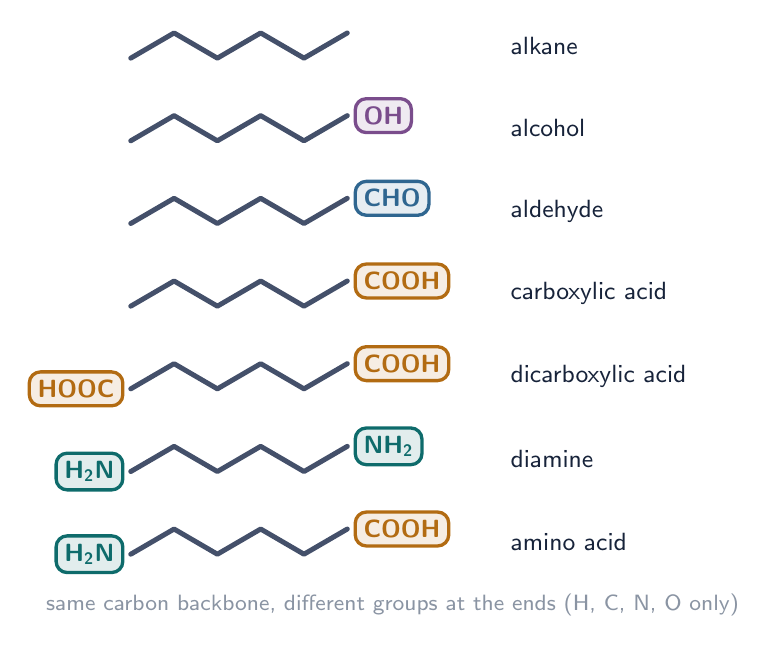
\begin{tikzpicture}
\draw[inksoft, line width=1.8pt] (1.90,-0.16) -- (2.45,0.16) -- (3.00,-0.16) -- (3.55,0.16) -- (4.10,-0.16) -- (4.65,0.16);
\node[font=\small, text=ink, anchor=west] at (6.6,0.00) {alkane};
\draw[inksoft, line width=1.8pt] (1.90,-1.21) -- (2.45,-0.89) -- (3.00,-1.21) -- (3.55,-0.89) -- (4.10,-1.21) -- (4.65,-0.89);
\node[draw=plum, fill=plum!12, line width=1.2pt, rounded corners=4pt, font=\small\bfseries, text=plum, anchor=west, inner sep=3pt] at (4.73,-0.89) {\ce{OH}};
\node[font=\small, text=ink, anchor=west] at (6.6,-1.05) {alcohol};
\draw[inksoft, line width=1.8pt] (1.90,-2.26) -- (2.45,-1.94) -- (3.00,-2.26) -- (3.55,-1.94) -- (4.10,-2.26) -- (4.65,-1.94);
\node[draw=blue, fill=blue!12, line width=1.2pt, rounded corners=4pt, font=\small\bfseries, text=blue, anchor=west, inner sep=3pt] at (4.73,-1.94) {\ce{CHO}};
\node[font=\small, text=ink, anchor=west] at (6.6,-2.10) {aldehyde};
\draw[inksoft, line width=1.8pt] (1.90,-3.31) -- (2.45,-2.99) -- (3.00,-3.31) -- (3.55,-2.99) -- (4.10,-3.31) -- (4.65,-2.99);
\node[draw=amber, fill=amber!12, line width=1.2pt, rounded corners=4pt, font=\small\bfseries, text=amber, anchor=west, inner sep=3pt] at (4.73,-2.99) {\ce{COOH}};
\node[font=\small, text=ink, anchor=west] at (6.6,-3.15) {carboxylic acid};
\draw[inksoft, line width=1.8pt] (1.90,-4.36) -- (2.45,-4.04) -- (3.00,-4.36) -- (3.55,-4.04) -- (4.10,-4.36) -- (4.65,-4.04);
\node[draw=amber, fill=amber!12, line width=1.2pt, rounded corners=4pt, font=\small\bfseries, text=amber, anchor=east, inner sep=3pt] at (1.82,-4.36) {\ce{HOOC}};
\node[draw=amber, fill=amber!12, line width=1.2pt, rounded corners=4pt, font=\small\bfseries, text=amber, anchor=west, inner sep=3pt] at (4.73,-4.04) {\ce{COOH}};
\node[font=\small, text=ink, anchor=west] at (6.6,-4.20) {dicarboxylic acid};
\draw[inksoft, line width=1.8pt] (1.90,-5.41) -- (2.45,-5.09) -- (3.00,-5.41) -- (3.55,-5.09) -- (4.10,-5.41) -- (4.65,-5.09);
\node[draw=teal, fill=teal!12, line width=1.2pt, rounded corners=4pt, font=\small\bfseries, text=teal, anchor=east, inner sep=3pt] at (1.82,-5.41) {\ce{H2N}};
\node[draw=teal, fill=teal!12, line width=1.2pt, rounded corners=4pt, font=\small\bfseries, text=teal, anchor=west, inner sep=3pt] at (4.73,-5.09) {\ce{NH2}};
\node[font=\small, text=ink, anchor=west] at (6.6,-5.25) {diamine};
\draw[inksoft, line width=1.8pt] (1.90,-6.46) -- (2.45,-6.14) -- (3.00,-6.46) -- (3.55,-6.14) -- (4.10,-6.46) -- (4.65,-6.14);
\node[draw=teal, fill=teal!12, line width=1.2pt, rounded corners=4pt, font=\small\bfseries, text=teal, anchor=east, inner sep=3pt] at (1.82,-6.46) {\ce{H2N}};
\node[draw=amber, fill=amber!12, line width=1.2pt, rounded corners=4pt, font=\small\bfseries, text=amber, anchor=west, inner sep=3pt] at (4.73,-6.14) {\ce{COOH}};
\node[font=\small, text=ink, anchor=west] at (6.6,-6.30) {amino acid};
\node[font=\footnotesize, text=greyc, anchor=west] at (0.7,-7.10) {same carbon backbone, different groups at the ends (H, C, N, O only)};
\end{tikzpicture}
\end{document}
